\section{Podstawowe parametry czasowe}
Podstawowym parametrem jest długość trwania tzw. \textit{cyklu wymian} czyli odcinka czasu, na którym pojawią się wszystkie wymiany konieczne dla sprawnego działania systemu. Jest on zazwyczaj ograniczony od góry wymaganiami czasowymi, jakie musi spełniać system aby kwalifikował się jako system czasu rzeczywistego.\\
W \textit{cyklu sieci} wyróżnić można pojedyncze \textit{wymiany}, które należą zazwyczaj do jednej z następujących kategorii:
\begin{itemize}
	\item \textit{zapytanie} bądź \textit{polecenie sterujące} wraz z odpowiedzią
	\item transmisja rozgłoszeniowa (w tego typu transmisji nie występują odpowiedzi od stacji slave)
\end{itemize}

	\subsection{Przebieg pojedynczej wymiany}
	Aby dowiedzieć się ile trwa cykl wymiany między stacją master a stacją slave, należy szczegółowo przeanalizować z jakich etapów składa się cykl wymiany i jak w wyniku tego należy sieć skonfigurować alby działała stabilnie i niezawodnie. Dwa podstawowe parametry, które mają na to wpływ to:
	\begin{itemize}
		\item Czas oczekiwania przez stację master na odpowiedź od stacji podrzędnej - $ T_{OODP} $
		\item Czas oczekiwania na gotowość stacji nadrzędnej -  $ T_{GOT} $
	\end{itemize}
	Rozważmy, co się stanie, jeśli powyższe czasy zostaną źle dobrane. \\ Za krótki czas $ T_{GOT} $ będzie powodował, że stacja slave notorycznie będzie zgłaszała brak gotowości stacji master i niemożność zrealizowania wymiany. \\
	Za krótki czas $ T_{OODP} $ będzie z kolei powodował częste komunikaty stacji master o braku połączenia ze stacją slave. \\
	Co więcej, powyższe parametry warto dobrać z pewnym marginesem, zabezpieczających nas od wszelakich opóźnień mogących wystąpić na etapie transmisji, bądź przetwarzania danych na granicy Jednostki Centralnej i Koprocesora Sieci.\\
	\\
	Przeanalizujmy co się dzieje w ciągu pojedynczej wymiany i jakie opóźnienia czasowe tam występują.\\
	Przede wszystkim jednostka centralna stacji master przekazuje do koprocesora informacje jakie żądanie musi zostać zrealizowane. Po zakończeniu cyklu automatu master musi zostać przygotowana ramka żądania, bo przecież abonent docelowy musi zostać zaadresowany, należy zapewnić kontrolę poprawności danych sumą CRC itp. Określimy ten czas jako $ T_{PZ} $. \\
	Przygotowaną ramkę, należy przesłać łączem fizycznym do abonenta docelowego - czas przesyłu jest bezpośrednio związany z właściwością łącza i ustaloną prędkością transmisji danych. Czas propagacji danych po łączu określimy jako $ T_{TRZ} $. Po wysłaniu ramki przez stację master, koprocesor docelowej stacji slave musi wykryć tą ramkę, i odczytać jej adres, bo przecież wcale nie musi być celem transmisji - jest to czas detekcji ramki $ T_{DZ} $. Po ustaleniu przez koprocesor, że przesłane żądanie ma być zrealizowane, należy żądanie przeanalizować, i poinformować jednostkę centralną jakie działania ma podjąć, bądź też jakie dane przygotować do transmisji - określmy ten czas jako $ T_{AZ} $. Po przekazaniu danych do jednostki centralnej musi się wykonać cykl automatu stacji slave, w którym dane zostaną przygotowane do transmisji do mastera, bądź zostanie wykonana czynność nakazana w otrzymanym żądaniu - czas cyklu można określić jako $ T_{CS} $.\\
	Po cyklu automatu następuje jakby "odwrócenie" procesu - stacja slave przygotowuje ramkę odpowiedzi, a master będzie ją odbierał. W skład tego procesu wejdą następujące czasy: czas przygotowania ramki odpowiedzi - $ T_{PO} $, czas transmisji ramki odpowiedzi - $ T_{TRO} $, czas detekcji ramki odpowiedzi - $ T_{DO} $, czas analizy ramki odpowiedzi - $ T_{AO} $ i wreszcie czas cyklu automatu stacji master, w którym nastąpi przetworzenie odpowiedzi oraz zapisanie informacji o wymianie zakończonej sukcesem do raportu - $ T_{CM} $.\\
	\begin{figure}[h]
		\centering
		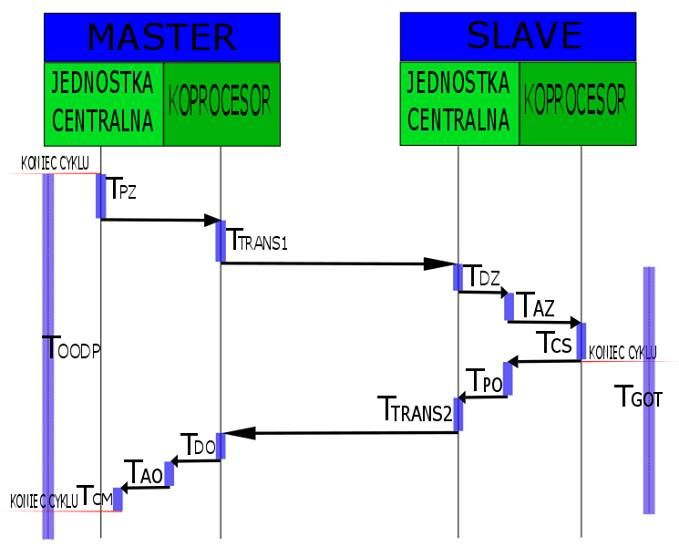
\includegraphics[width=0.7\textwidth]{./img/wymiana.jpg}
		\caption{Przebieg poszczególnych procesów podaczas pojedynczej wymiany}
		\label{fig:wymiana}
	\end{figure}
	\\
	Warto pamiętać, że dla poprawnej pracy sieci powinny zachodzić następujące zależności:
	\begin{equation}
		\label{eq:zalTgot}
		T_{GOT} > T_{DZ} + T_{AZ} + T_{CS} + T_{PO}
	\end{equation}
	\begin{equation}
		\label{eq:zalToodp}
		T_{OODP} > T_{PZ} + T_{TRZ} + T_{DZ} + T_{AZ} + T_{CS} + T_{PO} + T_{TRO} + T_{DO}
	\end{equation}
	Warto zwrócić uwagę na fakt, że w przypadku braku sygnału \textit{końca cyklu $ KC $} w czasie $ T_{GOT} $ koprocesor stacji slave wyśle odpowiedź $ NACK $ powodując uznanie wymiany za nieudaną. Jest to o tyle ważne, że wpływ na to ma czas trwania cyklu automatu slave $ T_{CS} $, którego długości nie da się wyliczyć, a jedynie zmierzyć. Dodatkowo będzie ona się prawdopodobnie zmieniała w zależności od działań podejmowanych przez stację slave, przez co może się drastycznie zmienić w wyniku komunikatów nadanych przez sieć. Takie zdarzenie może zaburzyć działanie sieci - dlatego należy doliczyć pewien margines w stosunku do przewidywanego najdłuższego czasu cyklu.
	
	\subsection{Analiza czasu trwania cyklu wymian}
	Na początek warto policzyć, ile czasu zajmie transmisja ramki przez łącze. Jest to dość proste, bo jest to stosunek liczby bitów w ramce do prędkości transmisji. Jedyne o czym należy pamiętać, to narzut bitów sterujących z protokołu.\\
	Czas transmisji ramki żądania:
	\begin{equation}
		\label{eq:czasTrz}
		T_{TRZ} = \frac{ZTZ*BZ + BS}{V[b/s]}
	\end{equation}
	Czas transmisji ramki odpowiedzi:
	\begin{equation}
		\label{eq:czasTro}
		T_{TRO} = \frac{ZTO*BZ+BS}{V[b/s]}
	\end{equation}
	Gdzie: $ ZTZ, ZTO $ to odpowiednio liczba znaków w danych w ramce żądania i odpowiedzi, $ BZ $ to liczba bitów w znaku, $ BS $ to liczba bitów sterujących narzucanych przez protokół (np. CRC itp.), a $ V $ to prędkość transmisji po łączu, wyrażana w $ bitach/sek $.\\
	\\
	Znając już czasy poszczególnych transmisji, można się zabrać za wyliczenie już bardziej złożonych rzeczy, jak choćby czasu trwania pojedynczej wymiany - jak łatwo się domyślić będzie to suma wszystkich składowych czasowych:
	\begin{equation}
		\label{eq:czasPW}
		T_{WYMP} = T_{PZ}+T_{TRZ} + T_{DZ} + T_{AZ} + T_{CS} + T_{PO} + T_{TRO} + T_{DO} + T_{AD} + T_{CM}
	\end{equation}
	Warto zwrócić uwagę, na fakt, że bardzo duży wpływ na czas trwania takiej wymiany mają cykle automatów mastera jak i slave'a. Dodatkowo są to parametry, które można zmienić w sposób dość prosty, gdyż nie wymaga to zmiany sprzętu. Natomiast zmiany parametrów detekcji ramki, czy analizy żądania bądź przygotowania odpowiedzi, są już zależne od użytego koprocesora i ich skrócenie wiązałoby się z koniecznością wymiany sprzętu.\\
	\\
	Kolejnym parametrem, który można sobie prosto wyliczyć jest czas trwania wszystkich $ N $ wymian:
	\begin{equation}
		\label{eq:czasWW}
		T_{WYMC} = \sum\limits_{i=1}^N (T_{PZi} + T_{TRZi}) + \sum\limits_{j=1}^N (T_{AZj} + T_{CSj} + T_{POj} + T_{TROj}) + \sum\limits_{i=1}^N (T_{CMi}+T_{T_{AOi}}) + N(T_{DZ} + T_{DO})
	\end{equation}
	Należy mieć na względzie, że wyliczone wyżej wartości zakładają brak jakichkolwiek retransmisji, usunięć z sieci stacji itd. Czas wykrycia niedostępności pojedynczego abonenta wynosi:
	\begin{equation}
		\label{eq:czasNiedost}
		T_{NA} = \sum\limits_{i=1}^{L_{REP}}(T_{TRZ} + T_{OODP})
	\end{equation}
	Jak widać, jest to czas powtórzenia $ L_{REP} $ razy transmisji wraz z oczekiwaniem na odpowiedź. Po upływie takiego czasu, stacja master uzna abonenta za niedostępnego i ponowi próbę komunikacji po wykonaniu się $ L_{COCZK} $ cykli sieci.\\
%	\begin{equation}
%		\label{eq:czasPO}
%		T_{POW} = \sum\limits_{i=1}^N L_{Ri}*T_{TRZi} + L_{Ri}T_{ODDP}
%	\end{equation}
	\\
	W najgorszym przypadku czas wszystkich transmisji będzie równy czasowi wszystkich transmisji + maksymalnemu czasowi repetycji, czyli:
	\begin{equation}
		\label{eq:czasMAX}
		T_{WYMMAX} = T_{WYMC} + \sum\limits_{i=1}^N T_{NAi}
	\end{equation}
\section{Poprawa parametrów sieci oraz jej modyfikacja}
	\subsection{Modyfikacja sieci}
		Każda sieć powinna obsługiwać podstawowe czynności związane z dodawaniem lub usuwaniem abonentów. Gdyby te dwa mechanizmy nie byłby dostępne to mogłaby by być po pewnym czasie cała sieć do wyrzucenia. Nie ma wtedy kontrolii nad błędami w systemie. W omawianym tutaj protokole jednak występują te dwa mechanizmy i dzięki nim możemy spokojnie rozszerzać naszą sieć bądź ją zmniejszać. A w razie awarii abonenta nie powinno dość do błędnej transmisji danych między resztą działających urządzeń
		\\
		\\
		 W MASTER-SLAVE pierwszy mechanizm jest realizowany w taki sposób, że to programista ma za zadanie ustalić na początku z jakimi abonentami ma być nawiązana transmisja (pod jakim adresem oni się znajdują) i w którą stronę ma odbywać się transmisja. Gdy już zostanie zdefiniowany scenariusz wymian, powinno zostać zapewnione połączenie fizyczne między slave'ami a masterem. Po uruchomieniu master wyśle ramkę rozgłoszeniową, a następnie sieć zacznie działać. W przypadku gdy chcielibyśmy dodać kolejnego abonenta do działającej już sieci, to jesteśmy zmuszeni do modyfikacji scenariusza wymian, aby slave został odpowiednio obsłużony. Jest to dosyć niewygodne rozwiązanie, ponieważ musimy przy każdej zmianie sprawdzać czy odpowiednie parametry działania sieci są poprawne. Być może dodanie kolejnego abonenta sprawi, że pojawią się błędne transmisje. 
		 \\
		 W jednym znanym zastosowaniu protokołu MASTER-SLAVE rozwiązano ten problem. Do każdego slave'a umieszczono pewną tablice danych zwanymi deskryptorami. Zawierają one informacje na temat obsługi danego slave'a. Master po wykryciu nowego slave'a po prostu wczytuje deskryptory i odpowiednio sam modyfikuje scenariusz wymian. Siecią o której teraz mowa jest popularne USB, które doczekało się już wersji 3.1 i nadal jest rozwijana. Popularność zapewne zawdzięcza temu mechanizmowi dodawania abonentów. Sprawia to, że taki system jest uniwersalny. 
		 \\
		 Innym rozwiązaniem, który można by było zastosować jest już w fazie projektowania umieszczenie dodatkowych "pustych" abonentów do sieci, których maksymalna ilość cykli sieci przy braku odpowiedzi oraz ilość prób nawiązania łączności będą na tyle duże, że w późniejszym czasie można będzie bez problemu wstawić brakującego slave'a. Jest to pewne rozwiązanie ale tu trzeba się zastanowić czy możemy sobie pozwolić na pogorszenie transmisji na rzecz rozbudowy systemu.
		\\
		\\
		Drugą wspomnianą czynnością edycji sieci jest usuwanie abonenta z niej. Ten mechanizm jest bardzo potrzebny żeby sieć działała cały czas sprawnie. Najczęstszym powodem usuwania abonenta z obiegu jest nie uzyskanie od niego odpowiedzi na wysłanego do niego zapytania. Spowodowane to może być błędami związanymi z transmisją albo po prostu uszkodzeniem abonenta. W protokole MASTER-SLAVE także wymyślony sposób usuwania nieobecnych slave'ów. Najpowszechniejszym rozwiązaniem jest ustalenie dwóch ważnych parametrów o których wcześniej wspominałem. Pierwszy z nich  to maksymalna liczba cykli sieci przy braku odpowiedzi. Przed ponownym wysłaniem ramki żądania do slave'a zostanie odczekana pewna liczba cykli sieci. Parametr ten poprawia znaczącą jakość działania sieci, ponieważ nie traci za każdym razem czasu na odpytywanie niedziałającego slave'a. Drugim parametrem jest ilość prób nawiązania łączności. Dzięki niemu po określonym czasie abonent zostanie po prostu wyrzucony z sieci (tzw. autousuwanie).
		